\section{Performance of parallel programs}

\subsection{More in-depth example showing utilization problems}

Note: will cover PARSEC/Splash2 in more detail in later section \cite{bienia2011benchmarking} \cite{bienia2008parsec} \cite{bienia2012characteristics}

\subsection{Performance without contention}

% TODO: replace with speed-up graph
\begin{figure}
\centering
  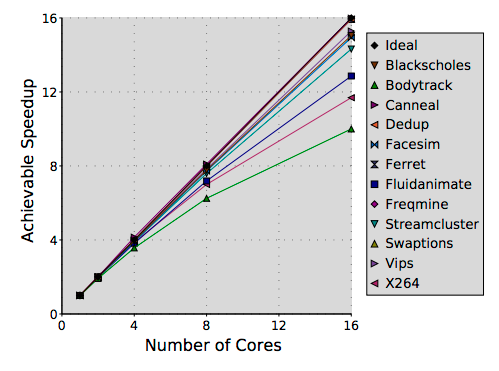
\includegraphics[width=8cm,height=4cm]{fig/speed-up.png}
  \caption{PLACEHOLDER: Wall-clock speed-up time. Upper bound for speedup of PARSEC workloads with input set simlarge based on instruction count. Limitations are caused by serial sections, growing parallelization overhead and redundant computations.}
  \label{fig:speed-up}
\end{figure}

% TODO: replace with slow-down total cpu time graph
\begin{figure}
\centering
  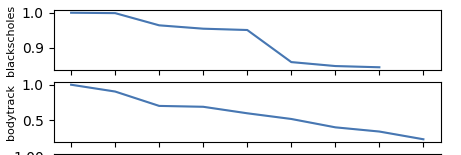
\includegraphics[width=8cm,height=4cm]{fig/slow-down.png}
  \caption{PLACEHOLDER: Although applications typically enjoy wall-clock speed-up times when they use more threads, often see corresponding increase in total CPU time [this graph might be confusing since we're talking about increase in total CPU time, but curve is going down]}
  \label{fig:slow-down}
\end{figure}

\begin{itemize}
  \item speed-up curve (see Figure \ref{fig:speed-up})
  \item slow-down curve (see Figure \ref{fig:slow-down})
\end{itemize}

\subsection{Performance under contention}

% TODO: replace with nicer figure for contention same
% TODO: need figure with mixed applications
\begin{figure}
\centering
  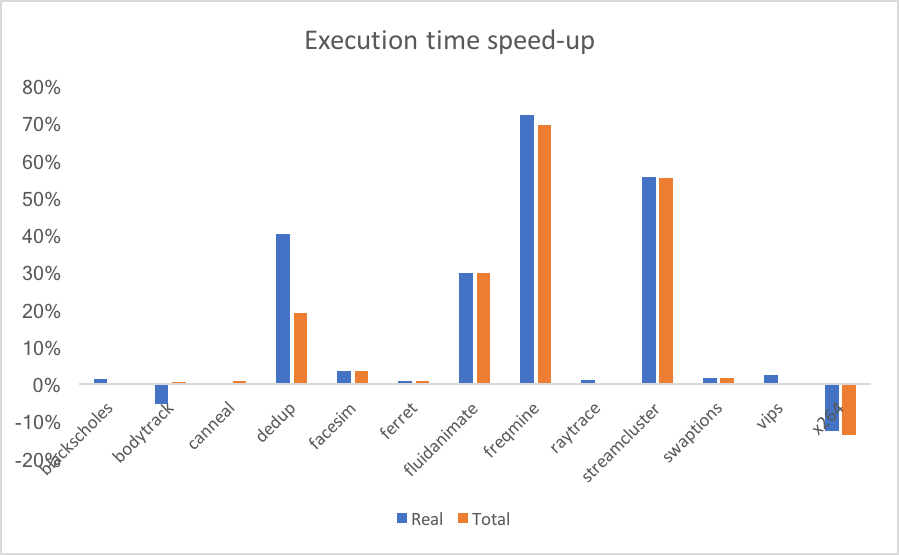
\includegraphics[width=8cm,height=4cm]{fig/contention-same.png}
  \caption{PLACEHOLDER: How groups of applications (same or mixed (need this fig)) do under contention at varying \# of threads}
  \label{fig:contention-same}
\end{figure}

\begin{itemize}
  \item same application (see Figure \ref{fig:contention-same})
  \item mixed group of applications (see Figure [])
\end{itemize}

\subsection{Reasons for contention}
\begin{itemize}
  \item thread contention (manny runnable threads, but divided work up into small pieces; not overlapping well with i/o)
  \item lock contention (why would this be exacerbated under contention?)
  \item other resource contention
\end{itemize}

\textbf{Classes of application behavior}
\begin{itemize}
  \item Big improvement from reducing parallelism (dedup, facesim, freqmine, streamcluster)
  \item Slight improvement from reducing parallelism
  \item Performance hit from reducing parallelism (x264)
\end{itemize}

\subsection{Common strategies for dealing with unknown resources}
TODO: maybe delete this section?
\begin{itemize}
  \item Overprovision number of threads and hope for the best. But this can cause problems (e.g., lock or resource contention)
\end{itemize}
